 \chapter{Dynamiques d'inflorescences et de larves pour le verger n\textdegree2}
 \label{chap:bloc2}
 
 Le verger n\textdegree2 présente des caractéristiques particulières qui impactent les résultats visibles.
 Ce verger est disposée «en escalier», avec une modalité sur chaque «marche».
 L'ensoleillement n'était pas le même entre les différentes modalités, et cela se ressent sur la figure~\ref{fig:inflos2}.
 La sous-parcelle avec un paillage synthétique --- la plus ensoleillé --- présente ainsi plus d'inflorescences que les deux autres.
 On retrouve aussi des différences d'inflorescences entre les parcelles enherbées, celle avec l'enherbement haut avait plus de soleil que l'autre, et elle a eu plus d'inflorescences.
 
 \begin{figure}[ht]
\centering
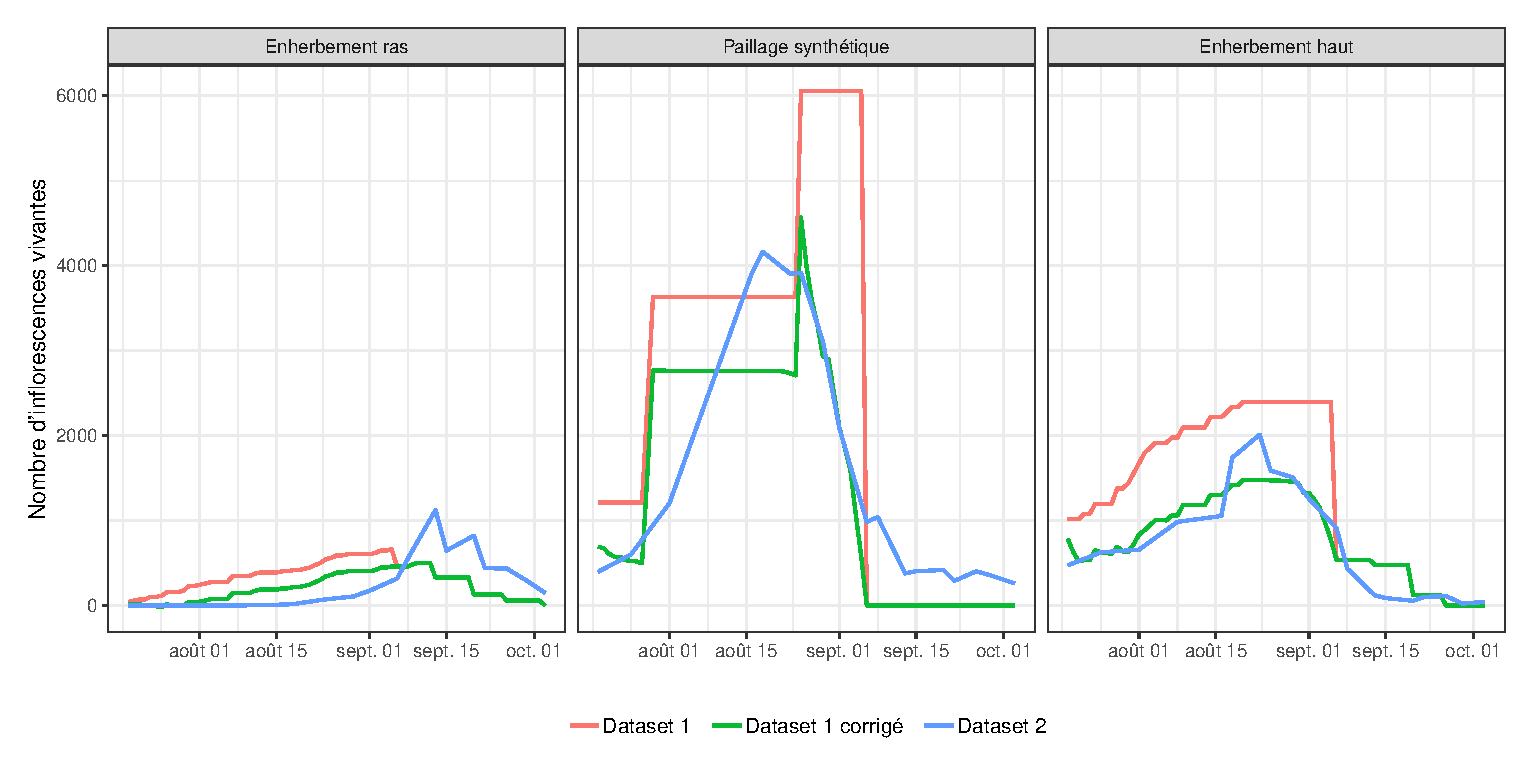
\epsfig{file = r/inflos_vivantes_bloc2.eps, scale = 0.59}
\caption{Comparaison des différentes dynamiques d'inflorescences vivantes du verger n\textdegree2 en fonction du \emph{dataset} utilisé. Même après correction, on observe des différences entre les dynamiques issues des différents jeu de données, en particulier pour les deux premières modalités.}
\label{fig:inflos2}
\end{figure}
\newpage
 On peut noter aussi des différences entre les deux jeux de données. C'est flagrant pour la modalité «paillage synthétique», où il n'y a seulement que 5 observations dans le \emph{dataset 1} produisant cette dynamique particulière. À cela se rajoute la variabilité du phénomène donnant des dynamiques très différentes pour des échantillonnages différents. Seule la sous-parcelle avec un enherbement haut présente des dynamiques similaires entre les deux jeux de données.
 
 Les dynamiques de larves pour ce verger sont visibles sur la figure~\ref{fig:larves2}.
 
 \begin{figure}[ht]
\centering
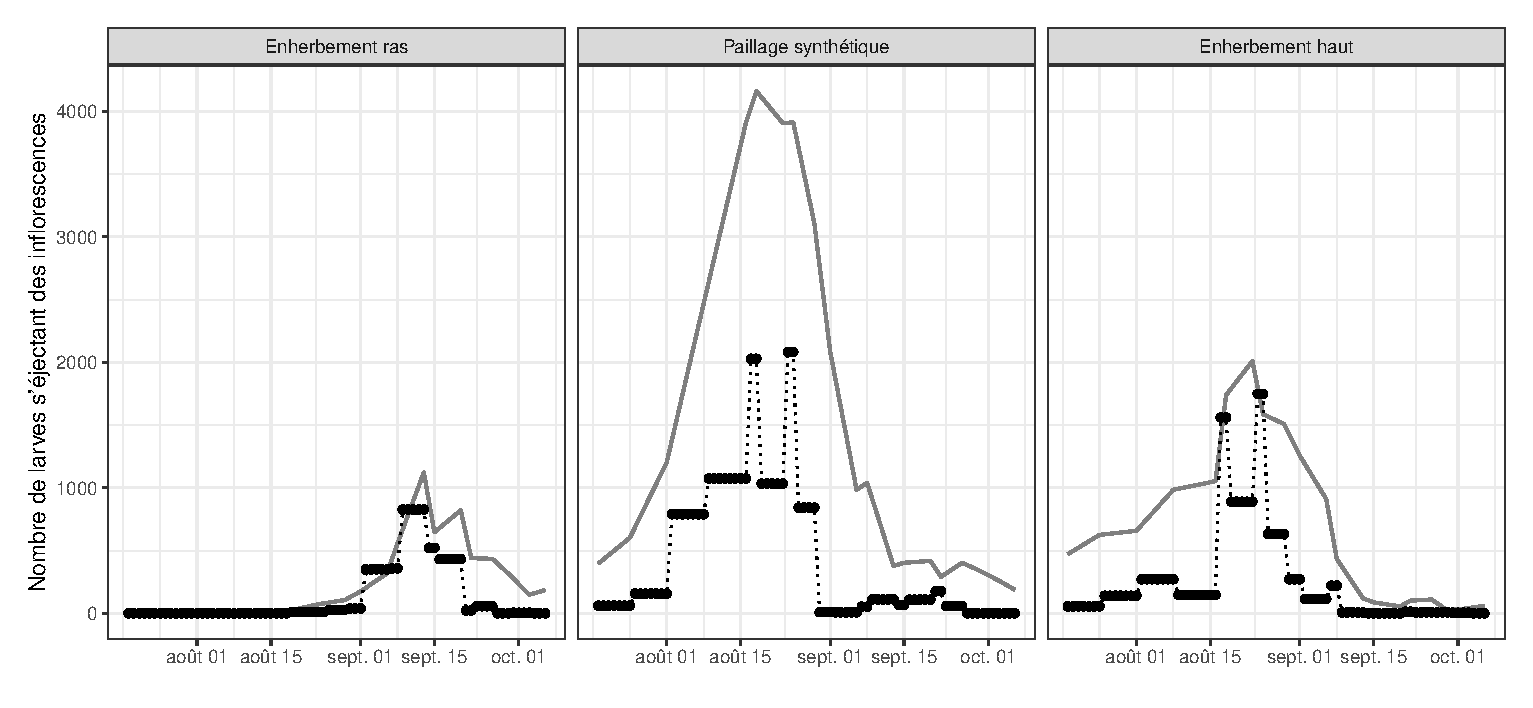
\epsfig{file = r/larves_bloc2.eps, scale = 0.59}
\caption{Dynamiques de larves s'éjectant des manguiers chaque jour dans le verger n\textdegree2 pour chacune des trois sous-parcelles. En gris sont visibles les dynamiques d'inflorescences vivantes.}
\label{fig:larves2}
\end{figure}

